%--coding: UTF-8 --
% !TEX program = xelatex
% 本模板由南开大学物理科学学院2018级本科生唐本豪制作,已通过XeLaTeX编译,允许修改和分发,且不必保留此声明,欢迎访问https://github.com/benhaotang/pubnotebook或邮件benhaotang@outlook.com一起开发和改进!
\documentclass{article}
\usepackage{ctexcap}
\usepackage{amsmath}
\usepackage{authblk}
\usepackage{graphicx}
\usepackage{fancyhdr}
\usepackage{multicol}
\usepackage{multicap}
\usepackage{tikz}
\newtheorem{theorem}{Theorem}
\newtheorem{lemma}{Lemma}
\newtheorem{proof}{Proof}[section]
\usetikzlibrary {optics}
\usetikzlibrary{shapes.geometric}
\fancyhf{}
\setlength{\textwidth}{474pt}
\setlength{\oddsidemargin}{-7pt}
\lhead{}\chead{}\rhead{}
\lfoot{}\cfoot{--\ \thepage\ --}\rfoot{}
\pagestyle{plain}
%标题行定义
\renewenvironment{abstract}{
	\textbf{摘要}:
}{\par}
\newenvironment{keyword}{
	\textbf{关键词}:
}{}
\newenvironment{entitle}{
\centering\normalfont\Huge
}{\par\vskip 1 cm}
\newenvironment{enauthor}{
\centering\normalfont\small
}{\par\vskip 0.25 cm}
\newenvironment{enaffil}{
\centering\normalfont\itshape\small
}{\par\vskip 0.25 cm}
\newenvironment{encal}{
	\centering\normalfont\small
}{\par}
\newenvironment{enabstract}{
	\textbf{Abstract}:
}{\par}
\newenvironment{enkeyword}{
	\textbf{Keywords}:
}{}
\title{\vspace{-30mm}\Huge\heiti 中文标题}
\author[1]{唐本豪}
\affil[1]{南开大学物理科学学院,天津 300110,中国}
\renewcommand*{\Affilfont}{\small\it}
\date{\today}
\begin{document}
\maketitle
\begin{abstract}
    这是一个论文模板
\end{abstract} 
\begin{keyword}
	\LaTeX{},论文写作
\end{keyword}
\begin{multicols}{2}
\section{正文}
\subsection{正文}
\subsubsection{正文}
从这里开始这里填写正文\par
\subsection{版权说明}
本模板由南开大学物理科学学院2018级本科生唐本豪制作,已通过XeLaTeX编译,允许修改和分发,且不必保留此声明\cite{web}欢迎访问https://github.com/benhaotang/pubnotebook一起开发和改进!同时,在使用这个模板的同时,如果遇到问题,也非常欢迎发送邮件至我的工作邮箱benhaotang@outlook.com一同交流!
\subsection{各个功能区块示例}
\subsubsection{公式}
\begin{equation}
    y = \left\{ \begin{array}{c}
        x^2\\
        \int^x_0{x^2}\\
        \text{无解}\\
    \end{array} \right.
\end{equation}
\subsubsection{表格}
\begin{center}
    \begin{tabular}{ccc}
        \hline
		A & A & A \\ \hline
		A & A & A \\ \hline
  \end{tabular}
  \label{tab:haha}
\end{center}
\subsubsection{Tikz绘图}
  \begin{center}
  
\begin{tikzpicture}
    \fill[red] (0,0) rectangle (7.5,5);
    \node[star,fill=yellow, minimum size=1.8cm, star point ratio=2.617,inner sep=0pt] at (1.3,3.6) {};
    \node[star,fill=yellow, minimum size=.5cm, rotate=30, star point ratio=2.617,inner sep=0pt] at (2.5,4.5) {};
    \node[star,fill=yellow, minimum size=.5cm, rotate=15, star point ratio=2.617,inner sep=0pt] at (3,3.9) {};
    \node[star,fill=yellow, minimum size=.5cm, rotate=0, star point ratio=2.617,inner sep=0pt] at (3,3.1) {};
    \node[star,fill=yellow, minimum size=.5cm, rotate=-15, star point ratio=2.617,inner sep=0pt] at (2.5,2.5) {};
  \end{tikzpicture}
  \mfcaption{中国国旗}
  \label{fig:flag}
\end{center}
\subsubsection{定理}
\begin{theorem}
这是一个定理!
\end{theorem}
由图\ref{fig:shiyi}接下来我们可以看到:
\begin{lemma}
这是一个引理!
\end{lemma}
我们来证明一下!
\begin{proof}
这是一个证明!
\end{proof}
\subsubsection{Tikz函数图像绘制}
  \begin{center}
    \scalebox{2}[1]{
        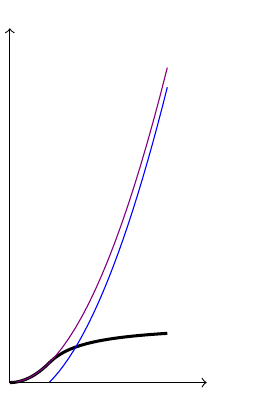
\begin{tikzpicture}
        \draw [black,domain=0:0.5,line width=1.1pt] plot(\x,\x*\x);
        \draw [black,domain=0.5:2,line width=1.1pt] plot(\x,-0.25*\x^-1+0.75) ;
        \draw [violet,domain=0:2] plot(\x,\x*\x) ;
        \draw [blue,domain=0.5:2] plot(\x,\x*\x-0.25) ;
        \draw [<->] (0,4.5) - - (0,0) - - (2.5,0) ;
        \end{tikzpicture}
        }
        \mfcaption{示意图}
        \label{fig:shiyi}
\end{center}
\par
我们来添加一个脚注吧\footnote{我支持香港警察,你们可以来打我了!},就像这样!
\section{感谢}
感谢您使用我的模板,谢谢!\par
大家一起努力,写出更加优秀的论文!为祖国的建设添砖加瓦!\par
\begin{thebibliography}{99}
    \bibitem{web} https://github.com/benhaotang/pubnotebook ,唐本豪的开放Github代码托管
\end{thebibliography}
\end{multicols}
\begin{entitle}
    English Title
\end{entitle} 
\begin{enauthor}
    Benhao Tang$^{1}$
\end{enauthor}
\begin{enaffil}
    $^{1}$School of Physics,Nankai University,Tianjin (300110),P.R.C
\end{enaffil}
\begin{encal}
    November 15,2019
\end{encal}
\begin{enabstract}
    This is a template for essay writing.
\end{enabstract}
\begin{enkeyword}
    \LaTeX{},Essay Writing
\end{enkeyword}  
\end{document} 